\documentclass[1p]{elsarticle_modified}
%\bibliographystyle{elsarticle-num}

%\usepackage[colorlinks]{hyperref}
%\usepackage{abbrmath_seonhwa} %\Abb, \Ascr, \Acal ,\Abf, \Afrak
\usepackage{amsfonts}
\usepackage{amssymb}
\usepackage{amsmath}
\usepackage{amsthm}
\usepackage{scalefnt}
\usepackage{amsbsy}
\usepackage{kotex}
\usepackage{caption}
\usepackage{subfig}
\usepackage{color}
\usepackage{graphicx}
\usepackage{xcolor} %% white, black, red, green, blue, cyan, magenta, yellow
\usepackage{float}
\usepackage{setspace}
\usepackage{hyperref}

\usepackage{tikz}
\usetikzlibrary{arrows}

\usepackage{multirow}
\usepackage{array} % fixed length table
\usepackage{hhline}

%%%%%%%%%%%%%%%%%%%%%
\makeatletter
\renewcommand*\env@matrix[1][\arraystretch]{%
	\edef\arraystretch{#1}%
	\hskip -\arraycolsep
	\let\@ifnextchar\new@ifnextchar
	\array{*\c@MaxMatrixCols c}}
\makeatother %https://tex.stackexchange.com/questions/14071/how-can-i-increase-the-line-spacing-in-a-matrix
%%%%%%%%%%%%%%%

\usepackage[normalem]{ulem}

\newcommand{\msout}[1]{\ifmmode\text{\sout{\ensuremath{#1}}}\else\sout{#1}\fi}
%SOURCE: \msout is \stkout macro in https://tex.stackexchange.com/questions/20609/strikeout-in-math-mode

\newcommand{\cancel}[1]{
	\ifmmode
	{\color{red}\msout{#1}}
	\else
	{\color{red}\sout{#1}}
	\fi
}

\newcommand{\add}[1]{
	{\color{blue}\uwave{#1}}
}

\newcommand{\replace}[2]{
	\ifmmode
	{\color{red}\msout{#1}}{\color{blue}\uwave{#2}}
	\else
	{\color{red}\sout{#1}}{\color{blue}\uwave{#2}}
	\fi
}

\newcommand{\Sol}{\mathcal{S}} %segment
\newcommand{\D}{D} %diagram
\newcommand{\A}{\mathcal{A}} %arc


%%%%%%%%%%%%%%%%%%%%%%%%%%%%%5 test

\def\sl{\operatorname{\textup{SL}}(2,\Cbb)}
\def\psl{\operatorname{\textup{PSL}}(2,\Cbb)}
\def\quan{\mkern 1mu \triangleright \mkern 1mu}

\theoremstyle{definition}
\newtheorem{thm}{Theorem}[section]
\newtheorem{prop}[thm]{Proposition}
\newtheorem{lem}[thm]{Lemma}
\newtheorem{ques}[thm]{Question}
\newtheorem{cor}[thm]{Corollary}
\newtheorem{defn}[thm]{Definition}
\newtheorem{exam}[thm]{Example}
\newtheorem{rmk}[thm]{Remark}
\newtheorem{alg}[thm]{Algorithm}

\newcommand{\I}{\sqrt{-1}}
\begin{document}

%\begin{frontmatter}
%
%\title{Boundary parabolic representations of knots up to 8 crossings}
%
%%% Group authors per affiliation:
%\author{Yunhi Cho} 
%\address{Department of Mathematics, University of Seoul, Seoul, Korea}
%\ead{yhcho@uos.ac.kr}
%
%
%\author{Seonhwa Kim} %\fnref{s_kim}}
%\address{Center for Geometry and Physics, Institute for Basic Science, Pohang, 37673, Korea}
%\ead{ryeona17@ibs.re.kr}
%
%\author{Hyuk Kim}
%\address{Department of Mathematical Sciences, Seoul National University, Seoul 08826, Korea}
%\ead{hyukkim@snu.ac.kr}
%
%\author{Seokbeom Yoon}
%\address{Department of Mathematical Sciences, Seoul National University, Seoul, 08826,  Korea}
%\ead{sbyoon15@snu.ac.kr}
%
%\begin{abstract}
%We find all boundary parabolic representation of knots up to 8 crossings.
%
%\end{abstract}
%\begin{keyword}
%    \MSC[2010] 57M25 
%\end{keyword}
%
%\end{frontmatter}

%\linenumbers
%\tableofcontents
%
\newcommand\colored[1]{\textcolor{white}{\rule[-0.35ex]{0.8em}{1.4ex}}\kern-0.8em\color{red} #1}%
%\newcommand\colored[1]{\textcolor{white}{ #1}\kern-2.17ex	\textcolor{white}{ #1}\kern-1.81ex	\textcolor{white}{ #1}\kern-2.15ex\color{red}#1	}

{\Large $\underline{12a_{0213}~(K12a_{0213})}$}

\setlength{\tabcolsep}{10pt}
\renewcommand{\arraystretch}{1.6}
\vspace{1cm}\begin{tabular}{m{100pt}>{\centering\arraybackslash}m{274pt}}
\multirow{5}{120pt}{
	\centering
	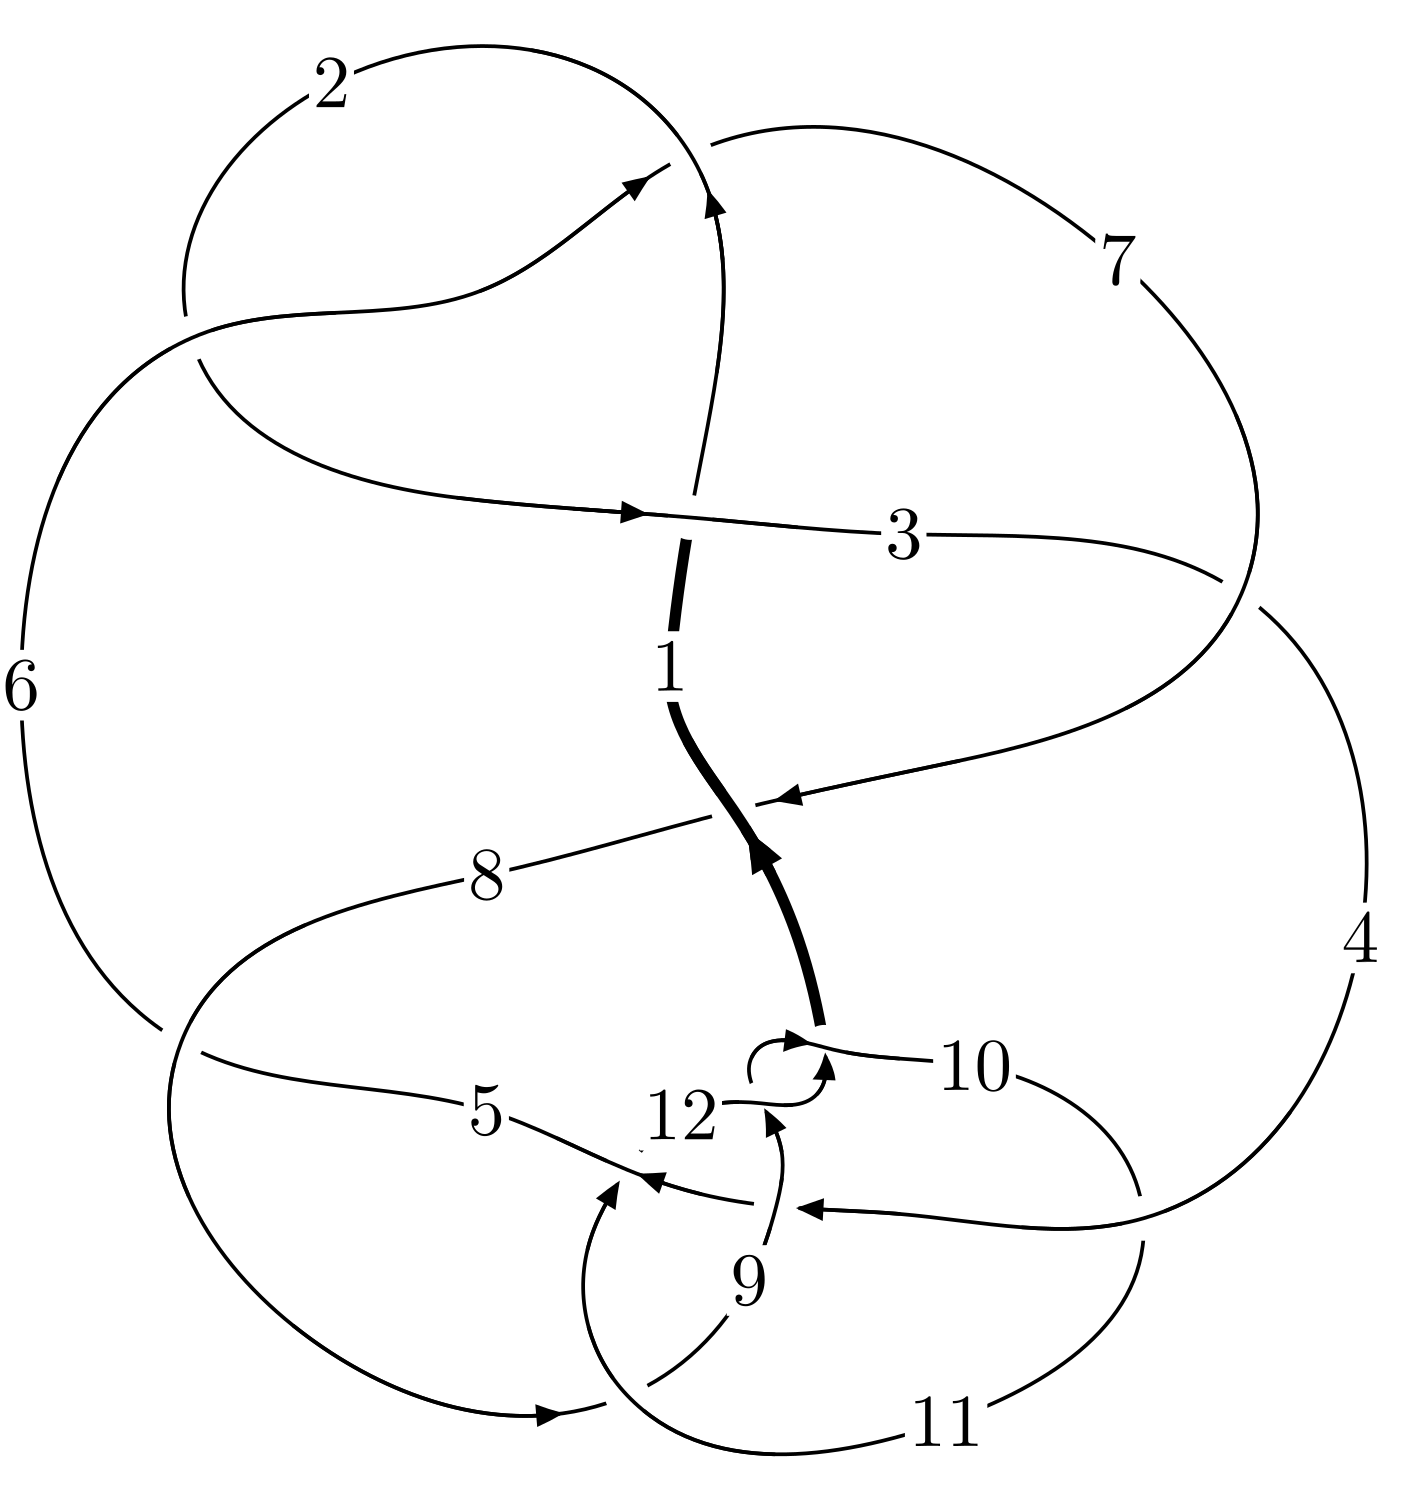
\includegraphics[width=112pt]{../../../GIT/diagram.site/Diagrams/png/1014_12a_0213.png}\\
\ \ \ A knot diagram\footnotemark}&
\allowdisplaybreaks
\textbf{Linearized knot diagam} \\
\cline{2-2}
 &
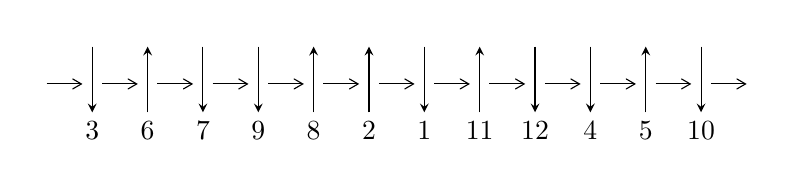
\begin{tikzpicture}[x=20pt, y=17pt]
	% nodes
	\node (C0) at (0, 0) {};
	\node (C1) at (1, 0) {};
	\node (C1U) at (1, +1) {};
	\node (C1D) at (1, -1) {3};

	\node (C2) at (2, 0) {};
	\node (C2U) at (2, +1) {};
	\node (C2D) at (2, -1) {6};

	\node (C3) at (3, 0) {};
	\node (C3U) at (3, +1) {};
	\node (C3D) at (3, -1) {7};

	\node (C4) at (4, 0) {};
	\node (C4U) at (4, +1) {};
	\node (C4D) at (4, -1) {9};

	\node (C5) at (5, 0) {};
	\node (C5U) at (5, +1) {};
	\node (C5D) at (5, -1) {8};

	\node (C6) at (6, 0) {};
	\node (C6U) at (6, +1) {};
	\node (C6D) at (6, -1) {2};

	\node (C7) at (7, 0) {};
	\node (C7U) at (7, +1) {};
	\node (C7D) at (7, -1) {1};

	\node (C8) at (8, 0) {};
	\node (C8U) at (8, +1) {};
	\node (C8D) at (8, -1) {11};

	\node (C9) at (9, 0) {};
	\node (C9U) at (9, +1) {};
	\node (C9D) at (9, -1) {12};

	\node (C10) at (10, 0) {};
	\node (C10U) at (10, +1) {};
	\node (C10D) at (10, -1) {4};

	\node (C11) at (11, 0) {};
	\node (C11U) at (11, +1) {};
	\node (C11D) at (11, -1) {5};

	\node (C12) at (12, 0) {};
	\node (C12U) at (12, +1) {};
	\node (C12D) at (12, -1) {10};
	\node (C13) at (13, 0) {};

	% arrows
	\draw[->,>={angle 60}]
	(C0) edge (C1) (C1) edge (C2) (C2) edge (C3) (C3) edge (C4) (C4) edge (C5) (C5) edge (C6) (C6) edge (C7) (C7) edge (C8) (C8) edge (C9) (C9) edge (C10) (C10) edge (C11) (C11) edge (C12) (C12) edge (C13) ;	\draw[->,>=stealth]
	(C1U) edge (C1D) (C2D) edge (C2U) (C3U) edge (C3D) (C4U) edge (C4D) (C5D) edge (C5U) (C6D) edge (C6U) (C7U) edge (C7D) (C8D) edge (C8U) (C9U) edge (C9D) (C10U) edge (C10D) (C11D) edge (C11U) (C12U) edge (C12D) ;
	\end{tikzpicture} \\
\hhline{~~} \\& 
\textbf{Solving Sequence} \\ \cline{2-2} 
 &
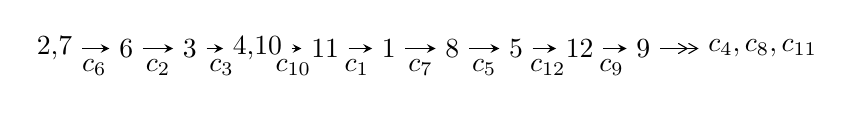
\begin{tikzpicture}[x=23pt, y=7pt]
	% node
	\node (A0) at (-1/8, 0) {2,7};
	\node (A1) at (1, 0) {6};
	\node (A2) at (2, 0) {3};
	\node (A3) at (49/16, 0) {4,10};
	\node (A4) at (33/8, 0) {11};
	\node (A5) at (41/8, 0) {1};
	\node (A6) at (49/8, 0) {8};
	\node (A7) at (57/8, 0) {5};
	\node (A8) at (65/8, 0) {12};
	\node (A9) at (73/8, 0) {9};
	\node (C1) at (1/2, -1) {$c_{6}$};
	\node (C2) at (3/2, -1) {$c_{2}$};
	\node (C3) at (5/2, -1) {$c_{3}$};
	\node (C4) at (29/8, -1) {$c_{10}$};
	\node (C5) at (37/8, -1) {$c_{1}$};
	\node (C6) at (45/8, -1) {$c_{7}$};
	\node (C7) at (53/8, -1) {$c_{5}$};
	\node (C8) at (61/8, -1) {$c_{12}$};
	\node (C9) at (69/8, -1) {$c_{9}$};
	\node (A10) at (11, 0) {$c_{4},c_{8},c_{11}$};

	% edge
	\draw[->,>=stealth]	
	(A0) edge (A1) (A1) edge (A2) (A2) edge (A3) (A3) edge (A4) (A4) edge (A5) (A5) edge (A6) (A6) edge (A7) (A7) edge (A8) (A8) edge (A9) ;
	\draw[->>,>={angle 60}]	
	(A9) edge (A10);
\end{tikzpicture} \\ 

\end{tabular} \\

\footnotetext{
The image of knot diagram is generated by the software ``\textbf{Draw programme}" developed by Andrew Bartholomew(\url{http://www.layer8.co.uk/maths/draw/index.htm\#Running-draw}), where we modified some parts for our purpose(\url{https://github.com/CATsTAILs/LinksPainter}).
}\phantom \\ \newline 
\centering \textbf{Ideals for irreducible components\footnotemark of $X_{\text{par}}$} 
 
\begin{align*}
I^u_{1}&=\langle 
-2.64097\times10^{40} u^{124}+4.69661\times10^{39} u^{123}+\cdots+3.19533\times10^{40} b-5.54363\times10^{39},\\
\phantom{I^u_{1}}&\phantom{= \langle  }9.07447\times10^{40} u^{124}+6.60265\times10^{40} u^{123}+\cdots+3.19533\times10^{40} a-5.09071\times10^{40},\;u^{125}+2 u^{124}+\cdots+u-1\rangle \\
I^u_{2}&=\langle 
b-1,\;a+2 u-1,\;u^2- u+1\rangle \\
\\
\end{align*}
\raggedright * 2 irreducible components of $\dim_{\mathbb{C}}=0$, with total 127 representations.\\
\footnotetext{All coefficients of polynomials are rational numbers. But the coefficients are sometimes approximated in decimal forms when there is not enough margin.}
\newpage
\renewcommand{\arraystretch}{1}
\centering \section*{I. $I^u_{1}= \langle -2.64\times10^{40} u^{124}+4.70\times10^{39} u^{123}+\cdots+3.20\times10^{40} b-5.54\times10^{39},\;9.07\times10^{40} u^{124}+6.60\times10^{40} u^{123}+\cdots+3.20\times10^{40} a-5.09\times10^{40},\;u^{125}+2 u^{124}+\cdots+u-1 \rangle$}
\flushleft \textbf{(i) Arc colorings}\\
\begin{tabular}{m{7pt} m{180pt} m{7pt} m{180pt} }
\flushright $a_{2}=$&$\begin{pmatrix}0\\u\end{pmatrix}$ \\
\flushright $a_{7}=$&$\begin{pmatrix}1\\0\end{pmatrix}$ \\
\flushright $a_{6}=$&$\begin{pmatrix}1\\u^2\end{pmatrix}$ \\
\flushright $a_{3}=$&$\begin{pmatrix}u\\u^3+u\end{pmatrix}$ \\
\flushright $a_{4}=$&$\begin{pmatrix}- u^3\\u^3+u\end{pmatrix}$ \\
\flushright $a_{10}=$&$\begin{pmatrix}-2.83992 u^{124}-2.06634 u^{123}+\cdots+4.13510 u+1.59317\\0.826508 u^{124}-0.146984 u^{123}+\cdots+1.45976 u+0.173492\end{pmatrix}$ \\
\flushright $a_{11}=$&$\begin{pmatrix}-1.24000 u^{124}-0.706679 u^{123}+\cdots+2.85485 u+1.83334\\0.266675 u^{124}+0.333348 u^{123}+\cdots+1.70001 u-0.0666735\end{pmatrix}$ \\
\flushright $a_{1}=$&$\begin{pmatrix}u^3\\u^5+u^3+u\end{pmatrix}$ \\
\flushright $a_{8}=$&$\begin{pmatrix}u^8+u^6+u^4+1\\u^{10}+2 u^8+3 u^6+2 u^4+u^2\end{pmatrix}$ \\
\flushright $a_{5}=$&$\begin{pmatrix}u^{16}+3 u^{14}+5 u^{12}+4 u^{10}+3 u^8+2 u^6+2 u^4+1\\u^{18}+4 u^{16}+9 u^{14}+12 u^{12}+11 u^{10}+6 u^8+2 u^6+u^2\end{pmatrix}$ \\
\flushright $a_{12}=$&$\begin{pmatrix}-2.64004 u^{124}-1.56683 u^{123}+\cdots+5.84349 u+1.44341\\0.726745 u^{124}-0.346510 u^{123}+\cdots+2.01012 u+0.273255\end{pmatrix}$ \\
\flushright $a_{9}=$&$\begin{pmatrix}-0.599959 u^{124}-1.83317 u^{123}+\cdots-3.19932 u+0.516585\\0.833251 u^{124}+1.66650 u^{123}+\cdots+0.949878 u-0.833252\end{pmatrix}$\\&\end{tabular}
\flushleft \textbf{(ii) Obstruction class $= -1$}\\~\\
\flushleft \textbf{(iii) Cusp Shapes $= 10.6193 u^{124}+2.39865 u^{123}+\cdots-23.1870 u+3.66068$}\\~\\
\newpage\renewcommand{\arraystretch}{1}
\flushleft \textbf{(iv) u-Polynomials at the component}\newline \\
\begin{tabular}{m{50pt}|m{274pt}}
Crossings & \hspace{64pt}u-Polynomials at each crossing \\
\hline $$\begin{aligned}c_{1}\end{aligned}$$&$\begin{aligned}
&u^{125}+60 u^{124}+\cdots+u-1
\end{aligned}$\\
\hline $$\begin{aligned}c_{2},c_{6}\end{aligned}$$&$\begin{aligned}
&u^{125}-2 u^{124}+\cdots+u+1
\end{aligned}$\\
\hline $$\begin{aligned}c_{3}\end{aligned}$$&$\begin{aligned}
&u^{125}+2 u^{124}+\cdots-16983 u+4113
\end{aligned}$\\
\hline $$\begin{aligned}c_{4}\end{aligned}$$&$\begin{aligned}
&u^{125}+4 u^{124}+\cdots- u-1
\end{aligned}$\\
\hline $$\begin{aligned}c_{5}\end{aligned}$$&$\begin{aligned}
&u^{125}+12 u^{124}+\cdots+5527915 u+76501
\end{aligned}$\\
\hline $$\begin{aligned}c_{7}\end{aligned}$$&$\begin{aligned}
&u^{125}-5 u^{124}+\cdots-1824 u+576
\end{aligned}$\\
\hline $$\begin{aligned}c_{8}\end{aligned}$$&$\begin{aligned}
&u^{125}+21 u^{124}+\cdots-4 u+4
\end{aligned}$\\
\hline $$\begin{aligned}c_{9},c_{12}\end{aligned}$$&$\begin{aligned}
&u^{125}-3 u^{124}+\cdots+4 u+1
\end{aligned}$\\
\hline $$\begin{aligned}c_{10}\end{aligned}$$&$\begin{aligned}
&u^{125}+40 u^{123}+\cdots+797687 u+83807
\end{aligned}$\\
\hline $$\begin{aligned}c_{11}\end{aligned}$$&$\begin{aligned}
&u^{125}+2 u^{124}+\cdots-94633 u+20921
\end{aligned}$\\
\hline
\end{tabular}\\~\\
\newpage\renewcommand{\arraystretch}{1}
\flushleft \textbf{(v) Riley Polynomials at the component}\newline \\
\begin{tabular}{m{50pt}|m{274pt}}
Crossings & \hspace{64pt}Riley Polynomials at each crossing \\
\hline $$\begin{aligned}c_{1}\end{aligned}$$&$\begin{aligned}
&y^{125}+12 y^{124}+\cdots+93 y-1
\end{aligned}$\\
\hline $$\begin{aligned}c_{2},c_{6}\end{aligned}$$&$\begin{aligned}
&y^{125}+60 y^{124}+\cdots+y-1
\end{aligned}$\\
\hline $$\begin{aligned}c_{3}\end{aligned}$$&$\begin{aligned}
&y^{125}-36 y^{124}+\cdots+355661613 y-16916769
\end{aligned}$\\
\hline $$\begin{aligned}c_{4}\end{aligned}$$&$\begin{aligned}
&y^{125}-20 y^{124}+\cdots+y-1
\end{aligned}$\\
\hline $$\begin{aligned}c_{5}\end{aligned}$$&$\begin{aligned}
&y^{125}+72 y^{124}+\cdots+18972461202289 y-5852403001
\end{aligned}$\\
\hline $$\begin{aligned}c_{7}\end{aligned}$$&$\begin{aligned}
&y^{125}+7 y^{124}+\cdots-23886720 y-331776
\end{aligned}$\\
\hline $$\begin{aligned}c_{8}\end{aligned}$$&$\begin{aligned}
&y^{125}+15 y^{124}+\cdots-312 y-16
\end{aligned}$\\
\hline $$\begin{aligned}c_{9},c_{12}\end{aligned}$$&$\begin{aligned}
&y^{125}-91 y^{124}+\cdots-80 y-1
\end{aligned}$\\
\hline $$\begin{aligned}c_{10}\end{aligned}$$&$\begin{aligned}
&y^{125}+80 y^{124}+\cdots-960105157739 y-7023613249
\end{aligned}$\\
\hline $$\begin{aligned}c_{11}\end{aligned}$$&$\begin{aligned}
&y^{125}+152 y^{124}+\cdots-25666758211 y-437688241
\end{aligned}$\\
\hline
\end{tabular}\\~\\
\newpage\flushleft \textbf{(vi) Complex Volumes and Cusp Shapes}
$$\begin{array}{c|c|c}  
\text{Solutions to }I^u_{1}& \I (\text{vol} + \sqrt{-1}CS) & \text{Cusp shape}\\
 \hline 
\begin{aligned}
u &= -0.679728 + 0.699024 I \\
a &= \phantom{-}0.120952 + 0.299129 I \\
b &= \phantom{-}1.057920 - 0.438992 I\end{aligned}
 & -1.66051 - 3.41079 I & \phantom{-0.000000 } 0 \\ \hline\begin{aligned}
u &= -0.679728 - 0.699024 I \\
a &= \phantom{-}0.120952 - 0.299129 I \\
b &= \phantom{-}1.057920 + 0.438992 I\end{aligned}
 & -1.66051 + 3.41079 I & \phantom{-0.000000 } 0 \\ \hline\begin{aligned}
u &= \phantom{-}0.417169 + 0.960639 I \\
a &= \phantom{-}0.06438 - 2.91642 I \\
b &= \phantom{-}1.48058 + 1.21311 I\end{aligned}
 & -3.43724 + 0.22308 I & \phantom{-0.000000 } 0 \\ \hline\begin{aligned}
u &= \phantom{-}0.417169 - 0.960639 I \\
a &= \phantom{-}0.06438 + 2.91642 I \\
b &= \phantom{-}1.48058 - 1.21311 I\end{aligned}
 & -3.43724 - 0.22308 I & \phantom{-0.000000 } 0 \\ \hline\begin{aligned}
u &= \phantom{-}0.042794 + 1.048360 I \\
a &= -0.93427 + 1.89066 I \\
b &= \phantom{-}0.499129 - 0.925280 I\end{aligned}
 & -3.55440 - 4.88679 I & \phantom{-0.000000 } 0 \\ \hline\begin{aligned}
u &= \phantom{-}0.042794 - 1.048360 I \\
a &= -0.93427 - 1.89066 I \\
b &= \phantom{-}0.499129 + 0.925280 I\end{aligned}
 & -3.55440 + 4.88679 I & \phantom{-0.000000 } 0 \\ \hline\begin{aligned}
u &= \phantom{-}0.527401 + 0.911523 I \\
a &= \phantom{-}0.83347 - 1.82848 I \\
b &= \phantom{-}0.323242 + 1.049860 I\end{aligned}
 & \phantom{-}0.87667 - 1.63345 I & \phantom{-0.000000 } 0 \\ \hline\begin{aligned}
u &= \phantom{-}0.527401 - 0.911523 I \\
a &= \phantom{-}0.83347 + 1.82848 I \\
b &= \phantom{-}0.323242 - 1.049860 I\end{aligned}
 & \phantom{-}0.87667 + 1.63345 I & \phantom{-0.000000 } 0 \\ \hline\begin{aligned}
u &= \phantom{-}0.654295 + 0.680316 I \\
a &= -0.249155 + 0.077471 I \\
b &= -1.84244 - 0.49259 I\end{aligned}
 & -2.79139 + 11.94370 I & \phantom{-0.000000 } 0 \\ \hline\begin{aligned}
u &= \phantom{-}0.654295 - 0.680316 I \\
a &= -0.249155 - 0.077471 I \\
b &= -1.84244 + 0.49259 I\end{aligned}
 & -2.79139 - 11.94370 I & \phantom{-0.000000 } 0\\
 \hline 
 \end{array}$$\newpage$$\begin{array}{c|c|c}  
\text{Solutions to }I^u_{1}& \I (\text{vol} + \sqrt{-1}CS) & \text{Cusp shape}\\
 \hline 
\begin{aligned}
u &= \phantom{-}0.588695 + 0.882150 I \\
a &= \phantom{-}0.62229 + 2.26840 I \\
b &= -1.382160 + 0.020555 I\end{aligned}
 & -3.39116 - 7.10514 I & \phantom{-0.000000 } 0 \\ \hline\begin{aligned}
u &= \phantom{-}0.588695 - 0.882150 I \\
a &= \phantom{-}0.62229 - 2.26840 I \\
b &= -1.382160 - 0.020555 I\end{aligned}
 & -3.39116 + 7.10514 I & \phantom{-0.000000 } 0 \\ \hline\begin{aligned}
u &= -0.302084 + 0.884500 I \\
a &= \phantom{-}1.315450 + 0.128898 I \\
b &= -0.350582 - 0.042146 I\end{aligned}
 & -0.17063 - 1.54245 I & \phantom{-0.000000 } 0 \\ \hline\begin{aligned}
u &= -0.302084 - 0.884500 I \\
a &= \phantom{-}1.315450 - 0.128898 I \\
b &= -0.350582 + 0.042146 I\end{aligned}
 & -0.17063 + 1.54245 I & \phantom{-0.000000 } 0 \\ \hline\begin{aligned}
u &= -0.632357 + 0.885540 I \\
a &= -0.657986 + 0.942609 I \\
b &= \phantom{-}0.893003 + 0.248469 I\end{aligned}
 & -2.20410 - 1.63394 I & \phantom{-0.000000 } 0 \\ \hline\begin{aligned}
u &= -0.632357 - 0.885540 I \\
a &= -0.657986 - 0.942609 I \\
b &= \phantom{-}0.893003 - 0.248469 I\end{aligned}
 & -2.20410 + 1.63394 I & \phantom{-0.000000 } 0 \\ \hline\begin{aligned}
u &= -0.481245 + 0.989878 I \\
a &= -2.15411 - 5.32330 I \\
b &= -1.79483 + 1.92968 I\end{aligned}
 & -1.99408 - 2.49462 I & \phantom{-0.000000 } 0 \\ \hline\begin{aligned}
u &= -0.481245 - 0.989878 I \\
a &= -2.15411 + 5.32330 I \\
b &= -1.79483 - 1.92968 I\end{aligned}
 & -1.99408 + 2.49462 I & \phantom{-0.000000 } 0 \\ \hline\begin{aligned}
u &= \phantom{-}0.614840 + 0.651355 I \\
a &= -0.202010 + 0.487116 I \\
b &= \phantom{-}1.083140 - 0.651367 I\end{aligned}
 & \phantom{-}1.63436 + 6.18286 I & \phantom{-0.000000 } 0 \\ \hline\begin{aligned}
u &= \phantom{-}0.614840 - 0.651355 I \\
a &= -0.202010 - 0.487116 I \\
b &= \phantom{-}1.083140 + 0.651367 I\end{aligned}
 & \phantom{-}1.63436 - 6.18286 I & \phantom{-0.000000 } 0\\
 \hline 
 \end{array}$$\newpage$$\begin{array}{c|c|c}  
\text{Solutions to }I^u_{1}& \I (\text{vol} + \sqrt{-1}CS) & \text{Cusp shape}\\
 \hline 
\begin{aligned}
u &= -0.523488 + 0.974857 I \\
a &= \phantom{-}0.535106 - 0.492195 I \\
b &= -0.180160 - 0.006470 I\end{aligned}
 & \phantom{-}0.13723 - 2.50988 I & \phantom{-0.000000 } 0 \\ \hline\begin{aligned}
u &= -0.523488 - 0.974857 I \\
a &= \phantom{-}0.535106 + 0.492195 I \\
b &= -0.180160 + 0.006470 I\end{aligned}
 & \phantom{-}0.13723 + 2.50988 I & \phantom{-0.000000 } 0 \\ \hline\begin{aligned}
u &= -0.714997 + 0.510109 I \\
a &= \phantom{-}0.136421 + 0.179960 I \\
b &= \phantom{-}1.06493 - 0.99596 I\end{aligned}
 & \phantom{-}1.69136 - 3.90937 I & \phantom{-0.000000 } 0 \\ \hline\begin{aligned}
u &= -0.714997 - 0.510109 I \\
a &= \phantom{-}0.136421 - 0.179960 I \\
b &= \phantom{-}1.06493 + 0.99596 I\end{aligned}
 & \phantom{-}1.69136 + 3.90937 I & \phantom{-0.000000 } 0 \\ \hline\begin{aligned}
u &= \phantom{-}0.560497 + 0.671639 I \\
a &= -0.212247 - 0.432133 I \\
b &= \phantom{-}1.86870 + 0.04556 I\end{aligned}
 & -2.79087 + 3.80135 I & \phantom{-0.000000 } 0 \\ \hline\begin{aligned}
u &= \phantom{-}0.560497 - 0.671639 I \\
a &= -0.212247 + 0.432133 I \\
b &= \phantom{-}1.86870 - 0.04556 I\end{aligned}
 & -2.79087 - 3.80135 I & \phantom{-0.000000 } 0 \\ \hline\begin{aligned}
u &= \phantom{-}0.455975 + 1.040590 I \\
a &= -0.820468 - 0.637657 I \\
b &= \phantom{-}1.48309 - 0.44923 I\end{aligned}
 & -4.48448 + 3.27623 I & \phantom{-0.000000 } 0 \\ \hline\begin{aligned}
u &= \phantom{-}0.455975 - 1.040590 I \\
a &= -0.820468 + 0.637657 I \\
b &= \phantom{-}1.48309 + 0.44923 I\end{aligned}
 & -4.48448 - 3.27623 I & \phantom{-0.000000 } 0 \\ \hline\begin{aligned}
u &= \phantom{-}0.730308 + 0.453581 I \\
a &= \phantom{-}0.061004 + 0.200975 I \\
b &= \phantom{-}0.70357 - 1.47380 I\end{aligned}
 & \phantom{-}1.41787 - 6.41870 I & \phantom{-0.000000 -}0. + 6.69453 I \\ \hline\begin{aligned}
u &= \phantom{-}0.730308 - 0.453581 I \\
a &= \phantom{-}0.061004 - 0.200975 I \\
b &= \phantom{-}0.70357 + 1.47380 I\end{aligned}
 & \phantom{-}1.41787 + 6.41870 I & \phantom{-0.000000 } 0. - 6.69453 I\\
 \hline 
 \end{array}$$\newpage$$\begin{array}{c|c|c}  
\text{Solutions to }I^u_{1}& \I (\text{vol} + \sqrt{-1}CS) & \text{Cusp shape}\\
 \hline 
\begin{aligned}
u &= \phantom{-}0.799477 + 0.308689 I \\
a &= \phantom{-}0.020614 + 0.223738 I \\
b &= \phantom{-}1.24228 - 1.00231 I\end{aligned}
 & -3.69917 - 5.73455 I & -6.85671 + 7.09378 I \\ \hline\begin{aligned}
u &= \phantom{-}0.799477 - 0.308689 I \\
a &= \phantom{-}0.020614 - 0.223738 I \\
b &= \phantom{-}1.24228 + 1.00231 I\end{aligned}
 & -3.69917 + 5.73455 I & -6.85671 - 7.09378 I \\ \hline\begin{aligned}
u &= -0.506487 + 1.025740 I \\
a &= \phantom{-}3.00969 + 3.23214 I \\
b &= \phantom{-}0.07486 - 2.30546 I\end{aligned}
 & -1.62403 - 3.30259 I & \phantom{-0.000000 } 0 \\ \hline\begin{aligned}
u &= -0.506487 - 1.025740 I \\
a &= \phantom{-}3.00969 - 3.23214 I \\
b &= \phantom{-}0.07486 + 2.30546 I\end{aligned}
 & -1.62403 + 3.30259 I & \phantom{-0.000000 } 0 \\ \hline\begin{aligned}
u &= -0.597525 + 0.607423 I \\
a &= \phantom{-}0.216601 + 0.430183 I \\
b &= -0.316208 + 0.286686 I\end{aligned}
 & \phantom{-}1.21505 - 1.94918 I & \phantom{-0.000000 -}0. + 2.49347 I \\ \hline\begin{aligned}
u &= -0.597525 - 0.607423 I \\
a &= \phantom{-}0.216601 - 0.430183 I \\
b &= -0.316208 - 0.286686 I\end{aligned}
 & \phantom{-}1.21505 + 1.94918 I & \phantom{-0.000000 } 0. - 2.49347 I \\ \hline\begin{aligned}
u &= \phantom{-}0.262991 + 1.120360 I \\
a &= \phantom{-}0.663394 - 1.183930 I \\
b &= -0.044368 + 1.250050 I\end{aligned}
 & -4.46336 - 0.92541 I & \phantom{-0.000000 } 0 \\ \hline\begin{aligned}
u &= \phantom{-}0.262991 - 1.120360 I \\
a &= \phantom{-}0.663394 + 1.183930 I \\
b &= -0.044368 - 1.250050 I\end{aligned}
 & -4.46336 + 0.92541 I & \phantom{-0.000000 } 0 \\ \hline\begin{aligned}
u &= -0.785970 + 0.311936 I \\
a &= -0.141515 + 0.120432 I \\
b &= -2.20613 - 1.49290 I\end{aligned}
 & -4.6627 + 14.1117 I & -2.00000 - 7.82782 I \\ \hline\begin{aligned}
u &= -0.785970 - 0.311936 I \\
a &= -0.141515 - 0.120432 I \\
b &= -2.20613 + 1.49290 I\end{aligned}
 & -4.6627 - 14.1117 I & -2.00000 + 7.82782 I\\
 \hline 
 \end{array}$$\newpage$$\begin{array}{c|c|c}  
\text{Solutions to }I^u_{1}& \I (\text{vol} + \sqrt{-1}CS) & \text{Cusp shape}\\
 \hline 
\begin{aligned}
u &= \phantom{-}0.308513 + 1.114810 I \\
a &= -1.68383 - 0.24557 I \\
b &= \phantom{-}1.46021 - 0.59103 I\end{aligned}
 & -4.94453 + 0.88598 I & \phantom{-0.000000 } 0 \\ \hline\begin{aligned}
u &= \phantom{-}0.308513 - 1.114810 I \\
a &= -1.68383 + 0.24557 I \\
b &= \phantom{-}1.46021 + 0.59103 I\end{aligned}
 & -4.94453 - 0.88598 I & \phantom{-0.000000 } 0 \\ \hline\begin{aligned}
u &= \phantom{-}0.285561 + 1.125560 I \\
a &= \phantom{-}4.55270 + 1.54514 I \\
b &= -3.76181 - 0.48262 I\end{aligned}
 & -6.48680 - 0.11053 I & \phantom{-0.000000 } 0 \\ \hline\begin{aligned}
u &= \phantom{-}0.285561 - 1.125560 I \\
a &= \phantom{-}4.55270 - 1.54514 I \\
b &= -3.76181 + 0.48262 I\end{aligned}
 & -6.48680 + 0.11053 I & \phantom{-0.000000 } 0 \\ \hline\begin{aligned}
u &= -0.256396 + 1.138060 I \\
a &= -2.30114 + 0.08256 I \\
b &= \phantom{-}1.43263 + 0.94921 I\end{aligned}
 & -4.43460 + 5.17173 I & \phantom{-0.000000 } 0 \\ \hline\begin{aligned}
u &= -0.256396 - 1.138060 I \\
a &= -2.30114 - 0.08256 I \\
b &= \phantom{-}1.43263 - 0.94921 I\end{aligned}
 & -4.43460 - 5.17173 I & \phantom{-0.000000 } 0 \\ \hline\begin{aligned}
u &= \phantom{-}0.458197 + 0.695142 I \\
a &= \phantom{-}0.27253 - 1.95867 I \\
b &= \phantom{-}0.965335 + 0.595467 I\end{aligned}
 & -3.15790 + 0.22084 I & -8.49031 - 0.86101 I \\ \hline\begin{aligned}
u &= \phantom{-}0.458197 - 0.695142 I \\
a &= \phantom{-}0.27253 + 1.95867 I \\
b &= \phantom{-}0.965335 - 0.595467 I\end{aligned}
 & -3.15790 - 0.22084 I & -8.49031 + 0.86101 I \\ \hline\begin{aligned}
u &= -0.278408 + 1.139920 I \\
a &= -2.84647 - 1.31941 I \\
b &= \phantom{-}1.15327 + 1.56068 I\end{aligned}
 & -8.80406 + 2.32103 I & \phantom{-0.000000 } 0 \\ \hline\begin{aligned}
u &= -0.278408 - 1.139920 I \\
a &= -2.84647 + 1.31941 I \\
b &= \phantom{-}1.15327 - 1.56068 I\end{aligned}
 & -8.80406 - 2.32103 I & \phantom{-0.000000 } 0\\
 \hline 
 \end{array}$$\newpage$$\begin{array}{c|c|c}  
\text{Solutions to }I^u_{1}& \I (\text{vol} + \sqrt{-1}CS) & \text{Cusp shape}\\
 \hline 
\begin{aligned}
u &= \phantom{-}0.507293 + 1.059410 I \\
a &= -2.35206 + 1.55375 I \\
b &= \phantom{-}0.37284 - 2.22618 I\end{aligned}
 & -2.52029 + 6.06447 I & \phantom{-0.000000 } 0 \\ \hline\begin{aligned}
u &= \phantom{-}0.507293 - 1.059410 I \\
a &= -2.35206 - 1.55375 I \\
b &= \phantom{-}0.37284 + 2.22618 I\end{aligned}
 & -2.52029 - 6.06447 I & \phantom{-0.000000 } 0 \\ \hline\begin{aligned}
u &= -0.297301 + 1.138330 I \\
a &= -0.456658 - 0.640099 I \\
b &= -0.259830 - 0.236853 I\end{aligned}
 & -9.01723 - 1.79866 I & \phantom{-0.000000 } 0 \\ \hline\begin{aligned}
u &= -0.297301 - 1.138330 I \\
a &= -0.456658 + 0.640099 I \\
b &= -0.259830 + 0.236853 I\end{aligned}
 & -9.01723 + 1.79866 I & \phantom{-0.000000 } 0 \\ \hline\begin{aligned}
u &= -0.322370 + 1.131930 I \\
a &= \phantom{-}1.349850 - 0.187015 I \\
b &= -0.795345 - 0.943236 I\end{aligned}
 & -5.16933 - 4.76940 I & \phantom{-0.000000 } 0 \\ \hline\begin{aligned}
u &= -0.322370 - 1.131930 I \\
a &= \phantom{-}1.349850 + 0.187015 I \\
b &= -0.795345 + 0.943236 I\end{aligned}
 & -5.16933 + 4.76940 I & \phantom{-0.000000 } 0 \\ \hline\begin{aligned}
u &= -0.757754 + 0.311437 I \\
a &= \phantom{-}0.054965 + 0.391931 I \\
b &= \phantom{-}1.99098 + 0.29231 I\end{aligned}
 & \phantom{-}0.00638 + 8.05941 I & -1.16635 - 7.77341 I \\ \hline\begin{aligned}
u &= -0.757754 - 0.311437 I \\
a &= \phantom{-}0.054965 - 0.391931 I \\
b &= \phantom{-}1.99098 - 0.29231 I\end{aligned}
 & \phantom{-}0.00638 - 8.05941 I & -1.16635 + 7.77341 I \\ \hline\begin{aligned}
u &= \phantom{-}0.556429 + 1.041740 I \\
a &= -0.34386 + 2.59385 I \\
b &= -1.61019 - 1.15977 I\end{aligned}
 & \phantom{-}2.38931 + 6.68336 I & \phantom{-0.000000 } 0 \\ \hline\begin{aligned}
u &= \phantom{-}0.556429 - 1.041740 I \\
a &= -0.34386 - 2.59385 I \\
b &= -1.61019 + 1.15977 I\end{aligned}
 & \phantom{-}2.38931 - 6.68336 I & \phantom{-0.000000 } 0\\
 \hline 
 \end{array}$$\newpage$$\begin{array}{c|c|c}  
\text{Solutions to }I^u_{1}& \I (\text{vol} + \sqrt{-1}CS) & \text{Cusp shape}\\
 \hline 
\begin{aligned}
u &= -0.538815 + 0.616206 I \\
a &= -2.15717 - 0.62315 I \\
b &= -2.66750 - 1.24723 I\end{aligned}
 & -0.88644 - 1.62714 I & \phantom{-}17.6831 - 19.5128 I \\ \hline\begin{aligned}
u &= -0.538815 - 0.616206 I \\
a &= -2.15717 + 0.62315 I \\
b &= -2.66750 + 1.24723 I\end{aligned}
 & -0.88644 + 1.62714 I & \phantom{-}17.6831 + 19.5128 I \\ \hline\begin{aligned}
u &= -0.242591 + 1.161340 I \\
a &= \phantom{-}2.94505 + 1.49559 I \\
b &= -1.60809 - 1.71649 I\end{aligned}
 & -9.2942 + 11.1311 I & \phantom{-0.000000 } 0 \\ \hline\begin{aligned}
u &= -0.242591 - 1.161340 I \\
a &= \phantom{-}2.94505 - 1.49559 I \\
b &= -1.60809 + 1.71649 I\end{aligned}
 & -9.2942 - 11.1311 I & \phantom{-0.000000 } 0 \\ \hline\begin{aligned}
u &= \phantom{-}0.653640 + 0.479882 I \\
a &= -0.174699 + 0.330105 I \\
b &= -1.61922 + 0.67646 I\end{aligned}
 & \phantom{-}4.03606 - 1.95840 I & \phantom{-}5.40020 + 2.12576 I \\ \hline\begin{aligned}
u &= \phantom{-}0.653640 - 0.479882 I \\
a &= -0.174699 - 0.330105 I \\
b &= -1.61922 - 0.67646 I\end{aligned}
 & \phantom{-}4.03606 + 1.95840 I & \phantom{-}5.40020 - 2.12576 I \\ \hline\begin{aligned}
u &= -0.596610 + 1.032710 I \\
a &= -1.54569 + 0.73226 I \\
b &= \phantom{-}1.158340 + 0.743651 I\end{aligned}
 & \phantom{-}0.152957 - 1.109810 I & \phantom{-0.000000 } 0 \\ \hline\begin{aligned}
u &= -0.596610 - 1.032710 I \\
a &= -1.54569 - 0.73226 I \\
b &= \phantom{-}1.158340 - 0.743651 I\end{aligned}
 & \phantom{-}0.152957 + 1.109810 I & \phantom{-0.000000 } 0 \\ \hline\begin{aligned}
u &= \phantom{-}0.738104 + 0.319751 I \\
a &= -0.062585 + 0.404238 I \\
b &= -0.547597 + 0.963150 I\end{aligned}
 & -0.13708 - 3.70904 I & -0.37034 + 1.40434 I \\ \hline\begin{aligned}
u &= \phantom{-}0.738104 - 0.319751 I \\
a &= -0.062585 - 0.404238 I \\
b &= -0.547597 - 0.963150 I\end{aligned}
 & -0.13708 + 3.70904 I & -0.37034 - 1.40434 I\\
 \hline 
 \end{array}$$\newpage$$\begin{array}{c|c|c}  
\text{Solutions to }I^u_{1}& \I (\text{vol} + \sqrt{-1}CS) & \text{Cusp shape}\\
 \hline 
\begin{aligned}
u &= \phantom{-}0.238691 + 1.173180 I \\
a &= -1.74345 + 1.16783 I \\
b &= \phantom{-}0.869383 - 1.084780 I\end{aligned}
 & -8.40775 - 2.68887 I & \phantom{-0.000000 } 0 \\ \hline\begin{aligned}
u &= \phantom{-}0.238691 - 1.173180 I \\
a &= -1.74345 - 1.16783 I \\
b &= \phantom{-}0.869383 + 1.084780 I\end{aligned}
 & -8.40775 + 2.68887 I & \phantom{-0.000000 } 0 \\ \hline\begin{aligned}
u &= -0.676930 + 0.423743 I \\
a &= \phantom{-}0.021492 + 0.350755 I \\
b &= -1.51090 - 0.16761 I\end{aligned}
 & \phantom{-}3.78834 - 0.01819 I & \phantom{-}5.34389 + 0.31518 I \\ \hline\begin{aligned}
u &= -0.676930 - 0.423743 I \\
a &= \phantom{-}0.021492 - 0.350755 I \\
b &= -1.51090 + 0.16761 I\end{aligned}
 & \phantom{-}3.78834 + 0.01819 I & \phantom{-}5.34389 - 0.31518 I \\ \hline\begin{aligned}
u &= -0.743871 + 0.288769 I \\
a &= -0.243464 - 0.168390 I \\
b &= \phantom{-}1.94501 + 1.38998 I\end{aligned}
 & -4.51308 + 5.31615 I & -7.83628 - 6.20055 I \\ \hline\begin{aligned}
u &= -0.743871 - 0.288769 I \\
a &= -0.243464 + 0.168390 I \\
b &= \phantom{-}1.94501 - 1.38998 I\end{aligned}
 & -4.51308 - 5.31615 I & -7.83628 + 6.20055 I \\ \hline\begin{aligned}
u &= -0.558215 + 1.072220 I \\
a &= \phantom{-}0.55939 - 2.37919 I \\
b &= -1.44362 + 0.58926 I\end{aligned}
 & \phantom{-}1.89272 - 4.76849 I & \phantom{-0.000000 } 0 \\ \hline\begin{aligned}
u &= -0.558215 - 1.072220 I \\
a &= \phantom{-}0.55939 + 2.37919 I \\
b &= -1.44362 - 0.58926 I\end{aligned}
 & \phantom{-}1.89272 + 4.76849 I & \phantom{-0.000000 } 0 \\ \hline\begin{aligned}
u &= -0.340644 + 1.163610 I \\
a &= \phantom{-}0.237640 - 0.493467 I \\
b &= \phantom{-}0.034493 + 1.011380 I\end{aligned}
 & -10.4687 - 10.1396 I & \phantom{-0.000000 } 0 \\ \hline\begin{aligned}
u &= -0.340644 - 1.163610 I \\
a &= \phantom{-}0.237640 + 0.493467 I \\
b &= \phantom{-}0.034493 - 1.011380 I\end{aligned}
 & -10.4687 + 10.1396 I & \phantom{-0.000000 } 0\\
 \hline 
 \end{array}$$\newpage$$\begin{array}{c|c|c}  
\text{Solutions to }I^u_{1}& \I (\text{vol} + \sqrt{-1}CS) & \text{Cusp shape}\\
 \hline 
\begin{aligned}
u &= \phantom{-}0.587202 + 1.067570 I \\
a &= \phantom{-}1.61895 - 1.96051 I \\
b &= \phantom{-}0.47226 + 1.69869 I\end{aligned}
 & -0.39121 + 11.44140 I & \phantom{-0.000000 } 0 \\ \hline\begin{aligned}
u &= \phantom{-}0.587202 - 1.067570 I \\
a &= \phantom{-}1.61895 + 1.96051 I \\
b &= \phantom{-}0.47226 - 1.69869 I\end{aligned}
 & -0.39121 - 11.44140 I & \phantom{-0.000000 } 0 \\ \hline\begin{aligned}
u &= \phantom{-}0.723221 + 0.295010 I \\
a &= -0.64670 - 1.32341 I \\
b &= -3.66740 - 0.92458 I\end{aligned}
 & -2.31097 - 3.02394 I & \phantom{-}15.4166 - 6.5863 I \\ \hline\begin{aligned}
u &= \phantom{-}0.723221 - 0.295010 I \\
a &= -0.64670 + 1.32341 I \\
b &= -3.66740 + 0.92458 I\end{aligned}
 & -2.31097 + 3.02394 I & \phantom{-}15.4166 + 6.5863 I \\ \hline\begin{aligned}
u &= \phantom{-}0.350810 + 1.173570 I \\
a &= -0.563732 - 0.198462 I \\
b &= \phantom{-}0.020877 + 0.351961 I\end{aligned}
 & -9.79515 + 1.43995 I & \phantom{-0.000000 } 0 \\ \hline\begin{aligned}
u &= \phantom{-}0.350810 - 1.173570 I \\
a &= -0.563732 + 0.198462 I \\
b &= \phantom{-}0.020877 - 0.351961 I\end{aligned}
 & -9.79515 - 1.43995 I & \phantom{-0.000000 } 0 \\ \hline\begin{aligned}
u &= -0.724995 + 0.268071 I \\
a &= -0.558292 - 0.965632 I \\
b &= -0.079967 + 0.440838 I\end{aligned}
 & -4.88103 + 1.27243 I & -8.99250 + 0.12894 I \\ \hline\begin{aligned}
u &= -0.724995 - 0.268071 I \\
a &= -0.558292 + 0.965632 I \\
b &= -0.079967 - 0.440838 I\end{aligned}
 & -4.88103 - 1.27243 I & -8.99250 - 0.12894 I \\ \hline\begin{aligned}
u &= \phantom{-}0.753049 + 0.147045 I \\
a &= -0.752425 + 0.367568 I \\
b &= \phantom{-}0.173370 + 0.028941 I\end{aligned}
 & -5.85796 - 2.23562 I & -10.68167 + 2.74645 I \\ \hline\begin{aligned}
u &= \phantom{-}0.753049 - 0.147045 I \\
a &= -0.752425 - 0.367568 I \\
b &= \phantom{-}0.173370 - 0.028941 I\end{aligned}
 & -5.85796 + 2.23562 I & -10.68167 - 2.74645 I\\
 \hline 
 \end{array}$$\newpage$$\begin{array}{c|c|c}  
\text{Solutions to }I^u_{1}& \I (\text{vol} + \sqrt{-1}CS) & \text{Cusp shape}\\
 \hline 
\begin{aligned}
u &= \phantom{-}0.536312 + 1.117790 I \\
a &= -1.40779 - 1.95839 I \\
b &= \phantom{-}2.14740 - 0.18715 I\end{aligned}
 & -3.39435 + 6.72398 I & \phantom{-0.000000 } 0 \\ \hline\begin{aligned}
u &= \phantom{-}0.536312 - 1.117790 I \\
a &= -1.40779 + 1.95839 I \\
b &= \phantom{-}2.14740 + 0.18715 I\end{aligned}
 & -3.39435 - 6.72398 I & \phantom{-0.000000 } 0 \\ \hline\begin{aligned}
u &= -0.739162 + 0.175015 I \\
a &= \phantom{-}0.771899 + 0.922373 I \\
b &= \phantom{-}0.067243 + 0.437011 I\end{aligned}
 & -6.51335 - 6.60957 I & -5.62101 + 4.12467 I \\ \hline\begin{aligned}
u &= -0.739162 - 0.175015 I \\
a &= \phantom{-}0.771899 - 0.922373 I \\
b &= \phantom{-}0.067243 - 0.437011 I\end{aligned}
 & -6.51335 + 6.60957 I & -5.62101 - 4.12467 I \\ \hline\begin{aligned}
u &= -0.524578 + 1.125060 I \\
a &= \phantom{-}1.08312 - 1.35457 I \\
b &= -1.69848 + 0.30164 I\end{aligned}
 & -3.80007 - 3.00363 I & \phantom{-0.000000 } 0 \\ \hline\begin{aligned}
u &= -0.524578 - 1.125060 I \\
a &= \phantom{-}1.08312 + 1.35457 I \\
b &= -1.69848 - 0.30164 I\end{aligned}
 & -3.80007 + 3.00363 I & \phantom{-0.000000 } 0 \\ \hline\begin{aligned}
u &= \phantom{-}0.546770 + 1.125950 I \\
a &= \phantom{-}3.64704 + 4.31957 I \\
b &= -3.93131 + 0.93753 I\end{aligned}
 & -4.71854 + 7.85425 I & \phantom{-0.000000 } 0 \\ \hline\begin{aligned}
u &= \phantom{-}0.546770 - 1.125950 I \\
a &= \phantom{-}3.64704 - 4.31957 I \\
b &= -3.93131 - 0.93753 I\end{aligned}
 & -4.71854 - 7.85425 I & \phantom{-0.000000 } 0 \\ \hline\begin{aligned}
u &= -0.539702 + 1.131940 I \\
a &= \phantom{-}0.464154 + 0.756708 I \\
b &= -0.478007 - 0.590823 I\end{aligned}
 & -7.37528 - 6.06661 I & \phantom{-0.000000 } 0 \\ \hline\begin{aligned}
u &= -0.539702 - 1.131940 I \\
a &= \phantom{-}0.464154 - 0.756708 I \\
b &= -0.478007 + 0.590823 I\end{aligned}
 & -7.37528 + 6.06661 I & \phantom{-0.000000 } 0\\
 \hline 
 \end{array}$$\newpage$$\begin{array}{c|c|c}  
\text{Solutions to }I^u_{1}& \I (\text{vol} + \sqrt{-1}CS) & \text{Cusp shape}\\
 \hline 
\begin{aligned}
u &= \phantom{-}0.557323 + 1.123800 I \\
a &= -0.75957 + 1.33123 I \\
b &= -0.73436 - 1.21005 I\end{aligned}
 & -2.48314 + 8.62396 I & \phantom{-0.000000 } 0 \\ \hline\begin{aligned}
u &= \phantom{-}0.557323 - 1.123800 I \\
a &= -0.75957 - 1.33123 I \\
b &= -0.73436 + 1.21005 I\end{aligned}
 & -2.48314 - 8.62396 I & \phantom{-0.000000 } 0 \\ \hline\begin{aligned}
u &= -0.508559 + 1.151200 I \\
a &= \phantom{-}0.612855 + 0.045245 I \\
b &= \phantom{-}0.467583 - 0.421339 I\end{aligned}
 & -9.32943 + 1.96630 I & \phantom{-0.000000 } 0 \\ \hline\begin{aligned}
u &= -0.508559 - 1.151200 I \\
a &= \phantom{-}0.612855 - 0.045245 I \\
b &= \phantom{-}0.467583 + 0.421339 I\end{aligned}
 & -9.32943 - 1.96630 I & \phantom{-0.000000 } 0 \\ \hline\begin{aligned}
u &= -0.549823 + 1.133070 I \\
a &= -0.00851 + 3.64990 I \\
b &= \phantom{-}2.09455 - 1.85308 I\end{aligned}
 & -6.97130 - 10.20430 I & \phantom{-0.000000 } 0 \\ \hline\begin{aligned}
u &= -0.549823 - 1.133070 I \\
a &= -0.00851 - 3.64990 I \\
b &= \phantom{-}2.09455 + 1.85308 I\end{aligned}
 & -6.97130 + 10.20430 I & \phantom{-0.000000 } 0 \\ \hline\begin{aligned}
u &= \phantom{-}0.681358 + 0.286026 I \\
a &= \phantom{-}0.643069 - 0.107415 I \\
b &= \phantom{-}1.57186 + 0.33127 I\end{aligned}
 & -1.01732 - 2.03022 I & -3.09406 + 4.57319 I \\ \hline\begin{aligned}
u &= \phantom{-}0.681358 - 0.286026 I \\
a &= \phantom{-}0.643069 + 0.107415 I \\
b &= \phantom{-}1.57186 - 0.33127 I\end{aligned}
 & -1.01732 + 2.03022 I & -3.09406 - 4.57319 I \\ \hline\begin{aligned}
u &= \phantom{-}0.499047 + 1.158250 I \\
a &= -0.487226 - 0.417308 I \\
b &= -0.0464337 + 0.1279410 I\end{aligned}
 & -8.78961 + 6.84987 I & \phantom{-0.000000 } 0 \\ \hline\begin{aligned}
u &= \phantom{-}0.499047 - 1.158250 I \\
a &= -0.487226 + 0.417308 I \\
b &= -0.0464337 - 0.1279410 I\end{aligned}
 & -8.78961 - 6.84987 I & \phantom{-0.000000 } 0\\
 \hline 
 \end{array}$$\newpage$$\begin{array}{c|c|c}  
\text{Solutions to }I^u_{1}& \I (\text{vol} + \sqrt{-1}CS) & \text{Cusp shape}\\
 \hline 
\begin{aligned}
u &= -0.560115 + 1.131450 I \\
a &= -1.19225 + 2.47759 I \\
b &= \phantom{-}2.39723 - 0.55290 I\end{aligned}
 & -2.39559 - 13.02930 I & \phantom{-0.000000 } 0 \\ \hline\begin{aligned}
u &= -0.560115 - 1.131450 I \\
a &= -1.19225 - 2.47759 I \\
b &= \phantom{-}2.39723 + 0.55290 I\end{aligned}
 & -2.39559 + 13.02930 I & \phantom{-0.000000 } 0 \\ \hline\begin{aligned}
u &= -0.530131 + 0.510836 I \\
a &= \phantom{-}0.772832 - 0.714498 I \\
b &= \phantom{-}0.53127 + 1.62919 I\end{aligned}
 & -0.099793 - 0.946670 I & -4.33653 + 4.47517 I \\ \hline\begin{aligned}
u &= -0.530131 - 0.510836 I \\
a &= \phantom{-}0.772832 + 0.714498 I \\
b &= \phantom{-}0.53127 - 1.62919 I\end{aligned}
 & -0.099793 + 0.946670 I & -4.33653 - 4.47517 I \\ \hline\begin{aligned}
u &= -0.568330 + 1.140120 I \\
a &= -0.11986 - 3.80079 I \\
b &= -2.38820 + 1.80200 I\end{aligned}
 & -7.1053 - 19.1835 I & \phantom{-0.000000 } 0 \\ \hline\begin{aligned}
u &= -0.568330 - 1.140120 I \\
a &= -0.11986 + 3.80079 I \\
b &= -2.38820 - 1.80200 I\end{aligned}
 & -7.1053 + 19.1835 I & \phantom{-0.000000 } 0 \\ \hline\begin{aligned}
u &= -0.683738 + 0.235270 I \\
a &= \phantom{-}0.016220 - 0.779945 I \\
b &= -1.108470 - 0.100376 I\end{aligned}
 & -1.28643 - 1.61583 I & -3.37728 + 3.87828 I \\ \hline\begin{aligned}
u &= -0.683738 - 0.235270 I \\
a &= \phantom{-}0.016220 + 0.779945 I \\
b &= -1.108470 + 0.100376 I\end{aligned}
 & -1.28643 + 1.61583 I & -3.37728 - 3.87828 I \\ \hline\begin{aligned}
u &= \phantom{-}0.570742 + 1.145300 I \\
a &= \phantom{-}0.19435 - 2.38956 I \\
b &= \phantom{-}1.34157 + 1.20026 I\end{aligned}
 & -6.17469 + 10.84830 I & \phantom{-0.000000 } 0 \\ \hline\begin{aligned}
u &= \phantom{-}0.570742 - 1.145300 I \\
a &= \phantom{-}0.19435 + 2.38956 I \\
b &= \phantom{-}1.34157 - 1.20026 I\end{aligned}
 & -6.17469 - 10.84830 I & \phantom{-0.000000 } 0\\
 \hline 
 \end{array}$$\newpage$$\begin{array}{c|c|c}  
\text{Solutions to }I^u_{1}& \I (\text{vol} + \sqrt{-1}CS) & \text{Cusp shape}\\
 \hline 
\begin{aligned}
u &= -0.122967 + 0.694323 I \\
a &= \phantom{-}1.248320 - 0.464863 I \\
b &= -0.377367 + 0.449759 I\end{aligned}
 & -0.15596 - 1.46517 I & -2.11111 + 4.06907 I \\ \hline\begin{aligned}
u &= -0.122967 - 0.694323 I \\
a &= \phantom{-}1.248320 + 0.464863 I \\
b &= -0.377367 - 0.449759 I\end{aligned}
 & -0.15596 + 1.46517 I & -2.11111 - 4.06907 I \\ \hline\begin{aligned}
u &= \phantom{-}0.529500 + 0.371661 I \\
a &= \phantom{-}0.750806 - 0.075379 I \\
b &= \phantom{-}0.14713 + 1.53695 I\end{aligned}
 & -0.59609 - 1.80402 I & -2.50103 + 5.03505 I \\ \hline\begin{aligned}
u &= \phantom{-}0.529500 - 0.371661 I \\
a &= \phantom{-}0.750806 + 0.075379 I \\
b &= \phantom{-}0.14713 - 1.53695 I\end{aligned}
 & -0.59609 + 1.80402 I & -2.50103 - 5.03505 I \\ \hline\begin{aligned}
u &= \phantom{-}0.299372\phantom{ +0.000000I} \\
a &= \phantom{-}3.72513\phantom{ +0.000000I} \\
b &= \phantom{-}0.723367\phantom{ +0.000000I}\end{aligned}
 & -2.39057\phantom{ +0.000000I} & -2.96710\phantom{ +0.000000I}\\
 \hline 
 \end{array}$$\newpage\newpage\renewcommand{\arraystretch}{1}
\centering \section*{II. $I^u_{2}= \langle b-1,\;a+2 u-1,\;u^2- u+1 \rangle$}
\flushleft \textbf{(i) Arc colorings}\\
\begin{tabular}{m{7pt} m{180pt} m{7pt} m{180pt} }
\flushright $a_{2}=$&$\begin{pmatrix}0\\u\end{pmatrix}$ \\
\flushright $a_{7}=$&$\begin{pmatrix}1\\0\end{pmatrix}$ \\
\flushright $a_{6}=$&$\begin{pmatrix}1\\u-1\end{pmatrix}$ \\
\flushright $a_{3}=$&$\begin{pmatrix}u\\u-1\end{pmatrix}$ \\
\flushright $a_{4}=$&$\begin{pmatrix}1\\u-1\end{pmatrix}$ \\
\flushright $a_{10}=$&$\begin{pmatrix}-2 u+1\\1\end{pmatrix}$ \\
\flushright $a_{11}=$&$\begin{pmatrix}- u+1\\0\end{pmatrix}$ \\
\flushright $a_{1}=$&$\begin{pmatrix}-1\\0\end{pmatrix}$ \\
\flushright $a_{8}=$&$\begin{pmatrix}1\\0\end{pmatrix}$ \\
\flushright $a_{5}=$&$\begin{pmatrix}- u+2\\u-1\end{pmatrix}$ \\
\flushright $a_{12}=$&$\begin{pmatrix}-2 u\\1\end{pmatrix}$ \\
\flushright $a_{9}=$&$\begin{pmatrix}1\\0\end{pmatrix}$\\&\end{tabular}
\flushleft \textbf{(ii) Obstruction class $= 1$}\\~\\
\flushleft \textbf{(iii) Cusp Shapes $= -4 u-1$}\\~\\
\newpage\renewcommand{\arraystretch}{1}
\flushleft \textbf{(iv) u-Polynomials at the component}\newline \\
\begin{tabular}{m{50pt}|m{274pt}}
Crossings & \hspace{64pt}u-Polynomials at each crossing \\
\hline $$\begin{aligned}c_{1},c_{3},c_{4}\\c_{5},c_{6},c_{10}\\c_{11}\end{aligned}$$&$\begin{aligned}
&u^2- u+1
\end{aligned}$\\
\hline $$\begin{aligned}c_{2}\end{aligned}$$&$\begin{aligned}
&u^2+u+1
\end{aligned}$\\
\hline $$\begin{aligned}c_{7},c_{8}\end{aligned}$$&$\begin{aligned}
&u^2
\end{aligned}$\\
\hline $$\begin{aligned}c_{9}\end{aligned}$$&$\begin{aligned}
&(u-1)^2
\end{aligned}$\\
\hline $$\begin{aligned}c_{12}\end{aligned}$$&$\begin{aligned}
&(u+1)^2
\end{aligned}$\\
\hline
\end{tabular}\\~\\
\newpage\renewcommand{\arraystretch}{1}
\flushleft \textbf{(v) Riley Polynomials at the component}\newline \\
\begin{tabular}{m{50pt}|m{274pt}}
Crossings & \hspace{64pt}Riley Polynomials at each crossing \\
\hline $$\begin{aligned}c_{1},c_{2},c_{3}\\c_{4},c_{5},c_{6}\\c_{10},c_{11}\end{aligned}$$&$\begin{aligned}
&y^2+y+1
\end{aligned}$\\
\hline $$\begin{aligned}c_{7},c_{8}\end{aligned}$$&$\begin{aligned}
&y^2
\end{aligned}$\\
\hline $$\begin{aligned}c_{9},c_{12}\end{aligned}$$&$\begin{aligned}
&(y-1)^2
\end{aligned}$\\
\hline
\end{tabular}\\~\\
\newpage\flushleft \textbf{(vi) Complex Volumes and Cusp Shapes}
$$\begin{array}{c|c|c}  
\text{Solutions to }I^u_{2}& \I (\text{vol} + \sqrt{-1}CS) & \text{Cusp shape}\\
 \hline 
\begin{aligned}
u &= \phantom{-}0.500000 + 0.866025 I \\
a &= \phantom{-0.000000 } -1.73205 I \\
b &= \phantom{-}1.00000\phantom{ +0.000000I}\end{aligned}
 & -1.64493 + 2.02988 I & -3.00000 - 3.46410 I \\ \hline\begin{aligned}
u &= \phantom{-}0.500000 - 0.866025 I \\
a &= \phantom{-0.000000 -}1.73205 I \\
b &= \phantom{-}1.00000\phantom{ +0.000000I}\end{aligned}
 & -1.64493 - 2.02988 I & -3.00000 + 3.46410 I\\
 \hline 
 \end{array}$$\newpage
\newpage\renewcommand{\arraystretch}{1}
\centering \section*{ III. u-Polynomials}
\begin{tabular}{m{50pt}|m{274pt}}
Crossings & \hspace{64pt}u-Polynomials at each crossing \\
\hline $$\begin{aligned}c_{1}\end{aligned}$$&$\begin{aligned}
&(u^2- u+1)(u^{125}+60 u^{124}+\cdots+u-1)
\end{aligned}$\\
\hline $$\begin{aligned}c_{2}\end{aligned}$$&$\begin{aligned}
&(u^2+u+1)(u^{125}-2 u^{124}+\cdots+u+1)
\end{aligned}$\\
\hline $$\begin{aligned}c_{3}\end{aligned}$$&$\begin{aligned}
&(u^2- u+1)(u^{125}+2 u^{124}+\cdots-16983 u+4113)
\end{aligned}$\\
\hline $$\begin{aligned}c_{4}\end{aligned}$$&$\begin{aligned}
&(u^2- u+1)(u^{125}+4 u^{124}+\cdots- u-1)
\end{aligned}$\\
\hline $$\begin{aligned}c_{5}\end{aligned}$$&$\begin{aligned}
&(u^2- u+1)(u^{125}+12 u^{124}+\cdots+5527915 u+76501)
\end{aligned}$\\
\hline $$\begin{aligned}c_{6}\end{aligned}$$&$\begin{aligned}
&(u^2- u+1)(u^{125}-2 u^{124}+\cdots+u+1)
\end{aligned}$\\
\hline $$\begin{aligned}c_{7}\end{aligned}$$&$\begin{aligned}
&u^2(u^{125}-5 u^{124}+\cdots-1824 u+576)
\end{aligned}$\\
\hline $$\begin{aligned}c_{8}\end{aligned}$$&$\begin{aligned}
&u^2(u^{125}+21 u^{124}+\cdots-4 u+4)
\end{aligned}$\\
\hline $$\begin{aligned}c_{9}\end{aligned}$$&$\begin{aligned}
&((u-1)^2)(u^{125}-3 u^{124}+\cdots+4 u+1)
\end{aligned}$\\
\hline $$\begin{aligned}c_{10}\end{aligned}$$&$\begin{aligned}
&(u^2- u+1)(u^{125}+40 u^{123}+\cdots+797687 u+83807)
\end{aligned}$\\
\hline $$\begin{aligned}c_{11}\end{aligned}$$&$\begin{aligned}
&(u^2- u+1)(u^{125}+2 u^{124}+\cdots-94633 u+20921)
\end{aligned}$\\
\hline $$\begin{aligned}c_{12}\end{aligned}$$&$\begin{aligned}
&((u+1)^2)(u^{125}-3 u^{124}+\cdots+4 u+1)
\end{aligned}$\\
\hline
\end{tabular}\newpage\renewcommand{\arraystretch}{1}
\centering \section*{ IV. Riley Polynomials}
\begin{tabular}{m{50pt}|m{274pt}}
Crossings & \hspace{64pt}Riley Polynomials at each crossing \\
\hline $$\begin{aligned}c_{1}\end{aligned}$$&$\begin{aligned}
&(y^2+y+1)(y^{125}+12 y^{124}+\cdots+93 y-1)
\end{aligned}$\\
\hline $$\begin{aligned}c_{2},c_{6}\end{aligned}$$&$\begin{aligned}
&(y^2+y+1)(y^{125}+60 y^{124}+\cdots+y-1)
\end{aligned}$\\
\hline $$\begin{aligned}c_{3}\end{aligned}$$&$\begin{aligned}
&(y^2+y+1)(y^{125}-36 y^{124}+\cdots+3.55662\times10^{8} y-1.69168\times10^{7})
\end{aligned}$\\
\hline $$\begin{aligned}c_{4}\end{aligned}$$&$\begin{aligned}
&(y^2+y+1)(y^{125}-20 y^{124}+\cdots+y-1)
\end{aligned}$\\
\hline $$\begin{aligned}c_{5}\end{aligned}$$&$\begin{aligned}
&(y^2+y+1)(y^{125}+72 y^{124}+\cdots+1.89725\times10^{13} y-5.85240\times10^{9})
\end{aligned}$\\
\hline $$\begin{aligned}c_{7}\end{aligned}$$&$\begin{aligned}
&y^2(y^{125}+7 y^{124}+\cdots-2.38867\times10^{7} y-331776)
\end{aligned}$\\
\hline $$\begin{aligned}c_{8}\end{aligned}$$&$\begin{aligned}
&y^2(y^{125}+15 y^{124}+\cdots-312 y-16)
\end{aligned}$\\
\hline $$\begin{aligned}c_{9},c_{12}\end{aligned}$$&$\begin{aligned}
&((y-1)^2)(y^{125}-91 y^{124}+\cdots-80 y-1)
\end{aligned}$\\
\hline $$\begin{aligned}c_{10}\end{aligned}$$&$\begin{aligned}
&(y^2+y+1)(y^{125}+80 y^{124}+\cdots-9.60105\times10^{11} y-7.02361\times10^{9})
\end{aligned}$\\
\hline $$\begin{aligned}c_{11}\end{aligned}$$&$\begin{aligned}
&(y^2+y+1)(y^{125}+152 y^{124}+\cdots-2.56668\times10^{10} y-4.37688\times10^{8})
\end{aligned}$\\
\hline
\end{tabular}
\vskip 2pc
\end{document}